\begin{figure}[h!]
  \centering
  \begin{subfigure}{0.45\linewidth}
    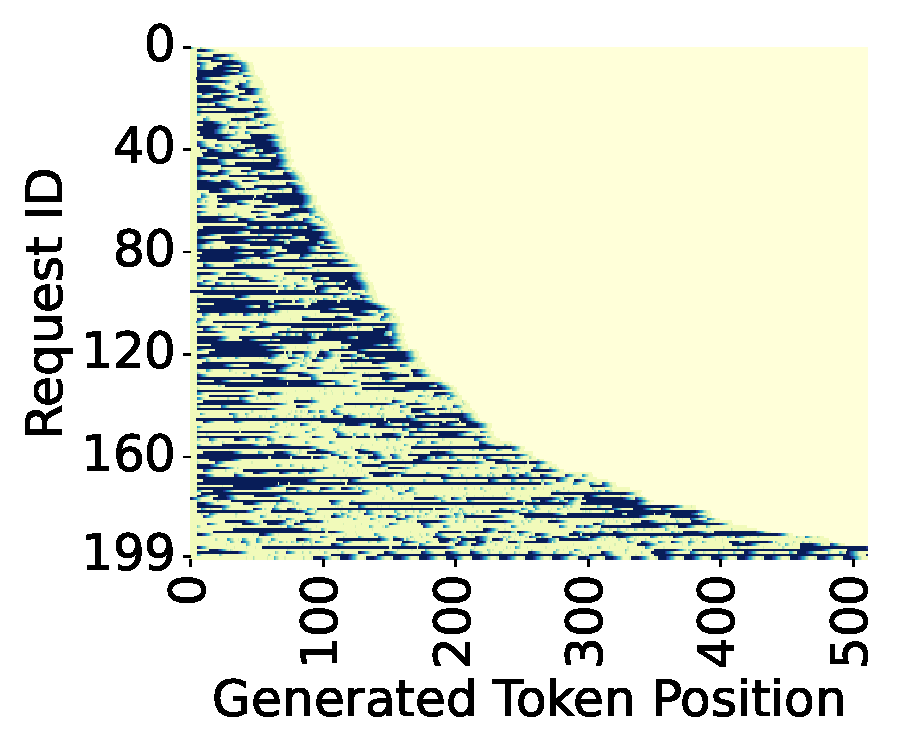
\includegraphics[width=\linewidth]{figures/acc_len/heatmap/instructcoder_ngram_llama3.1-8B_acceptance_stats.pdf}
    \caption{InstructCoder, $n$-gram}
  \end{subfigure}
  \hspace{1pt}
  \begin{subfigure}{0.45\linewidth}
    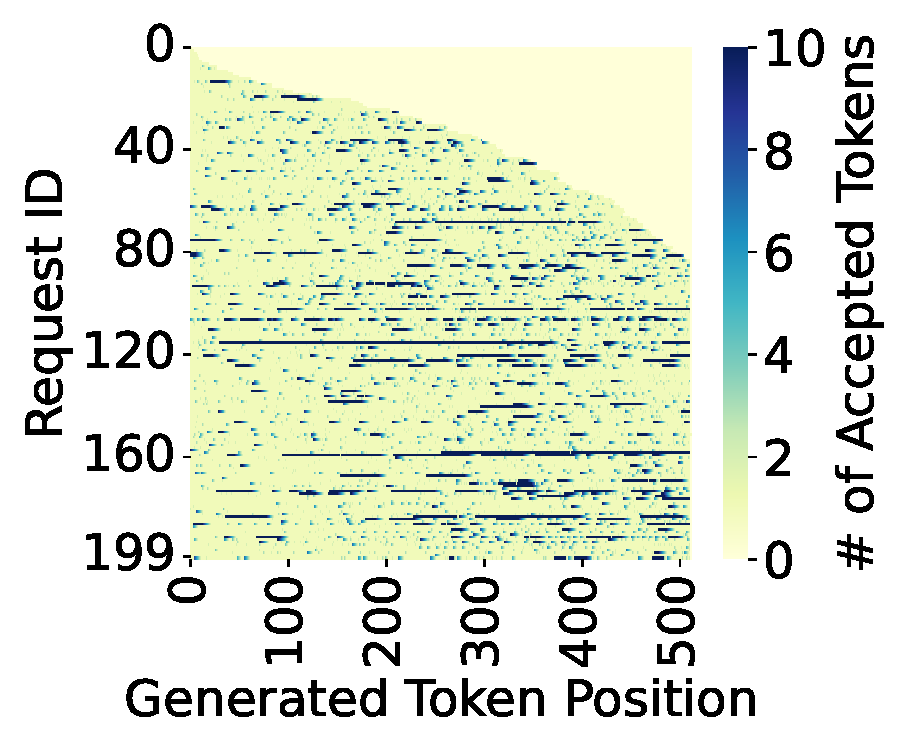
\includegraphics[width=\linewidth]{figures/acc_len/heatmap/sharegpt_ngram_llama3.1-8B_acceptance_stats.pdf}
    \caption{ShareGPT, $n$-gram}
  \end{subfigure}

   \begin{subfigure}{0.45\linewidth}
    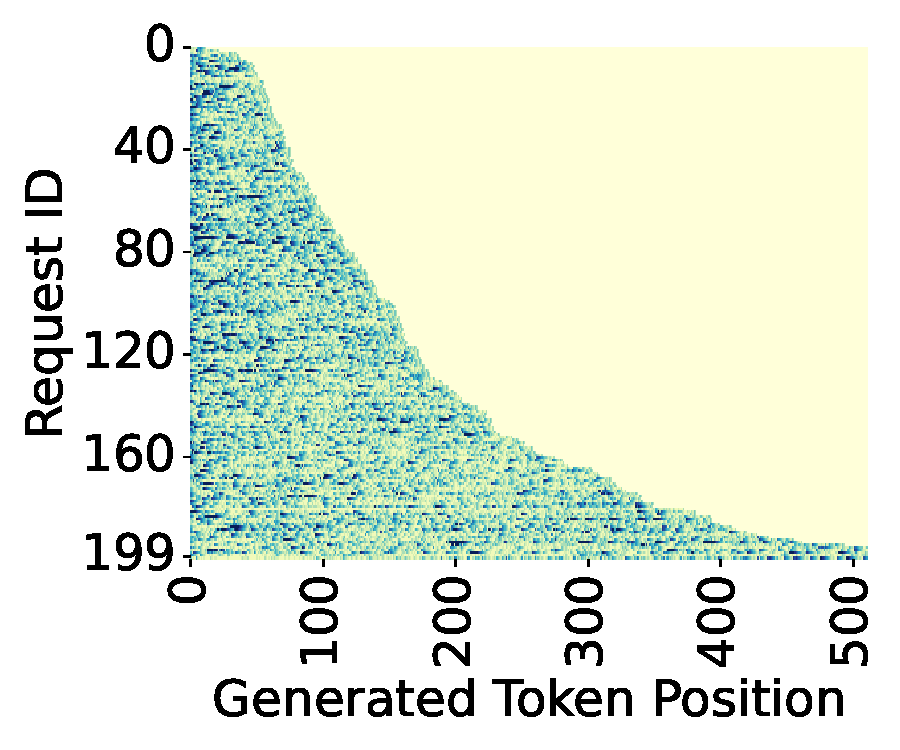
\includegraphics[width=\linewidth]{figures/acc_len/heatmap/instructcoder_eagle_llama3.1-8B_acceptance_stats.pdf}
    \caption{InstructCoder, EAGLE}
  \end{subfigure}
  \hspace{1pt}
  \begin{subfigure}{0.45\linewidth}
    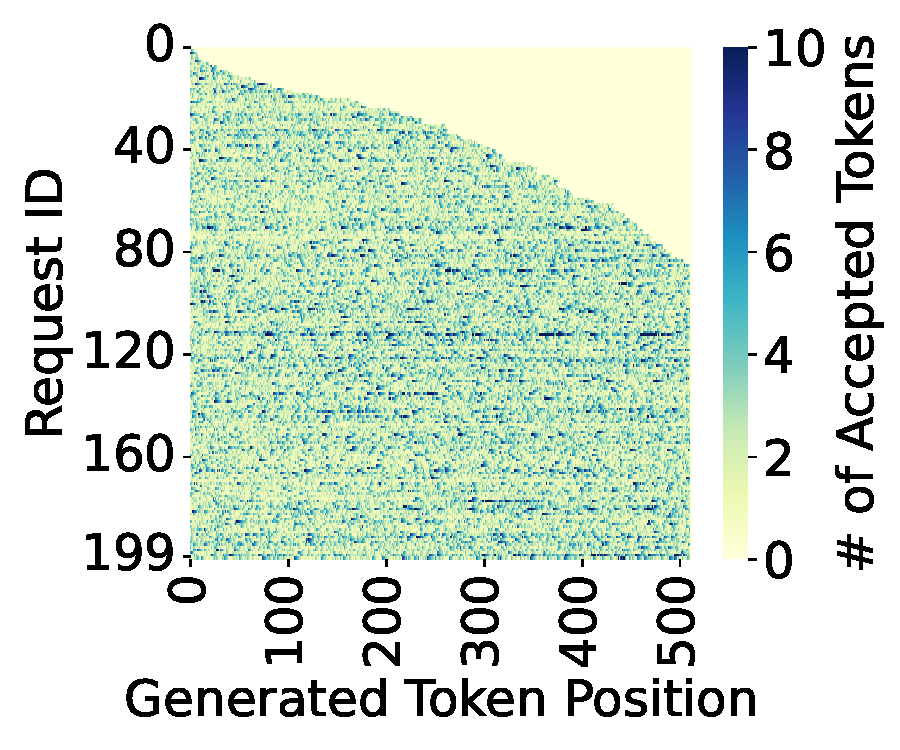
\includegraphics[width=\linewidth]{figures/acc_len/heatmap/sharegpt_eagle_llama3.1-8B_acceptance_stats.pdf}
    \caption{ShareGPT, EAGLE}
  \end{subfigure}

  \caption{Generation length per token position for Llama3.1-8B. Requests are sorted based on generation length. Darker colors indicate that more tokens are generated at the corresponding position.}
  \label{fig:acceptance-length-heatmap}
\end{figure}



\section{Acceptance Behavior}
\label{sec:acc-behavior}
To understand the acceptance rate, we measure the number of draft tokens generated\footnote{Number of generated tokens = accepted tokens proposed by the drafting method + 1 bonus token. Similarly, for generation length, it is computed by adding the acceptance length by one.} by the target model at each decoding step. 
For each dataset, we sample up to 200 requests. Each SD method proposes up to 20 tokens per step, and we record how many of these are generated at that step.  
After each generation step, even if multiple tokens were generated, we discard all but one and advance to the next position. 
Essentially, we approximate the maximum number of tokens that could be accepted at each generation step.
We analyze results for two non-reasoning models (Llama-3-70B and Llama-3.1-8B; max 512 output tokens) and one reasoning model (Qwen-3-8B-Thinking; max 32K output tokens).


\autoref{fig:acceptance-length-heatmap} visualizes the number of tokens generated at each output position for InstructCoder and ShareGPT (notice SD generates at least one token at each position, even if all proposed tokens are rejected). Each row represents a sampled request and each column a generation position, with color indicating the number of tokens produced by SD. 

\begin{quoting}[leftmargin=1.5em, rightmargin=1.5em, vskip=0pt]
\textbf{Summary.}
\emph{We observe the variance of generated token lengths along three dimensions: within a single request, across requests, and across datasets.}
\end{quoting}
\autoref{fig:acceptance-length-heatmap} gives a high level feeling of the generation length at each position across requests. $n$-grams and EAGLE show different patterns. $n$-grams show high variance, lots of very dark and very light positions, some positions generate a lot, while others only generate one. EAGLE show good average generation length (averge color is darker) and also less variance. But there are variance across all dimentions, which we will describe in more detail below. 


% Acceptance varies notably across positions (horizontal), requests (vertical), and datasets: within a request, acceptance fluctuates along the sequence; across requests, some are consistently easier to speculate than others; across datasets, for example, \autoref{fig:acceptance-length-heatmap} shows InstructCoder generally achieves higher acceptance (darker) than ShareGPT.

% \autoref{fig:acceptance-length-heatmap} presents the number of generated tokens (notice SD generates at least one token at each position, even if all proposed tokens are rejected) at each generation position for InstructCoder and ShareGPT. Each row corresponds to one sampled request, and each column to a generation position, with color indicating the number of tokens generated by SD\footnote{Number of generated tokens = number of accepted tokens proposed by the drafting method + 1}.
% As shown, acceptance behavior exhibits \textbf{significant variance} across positions (horizontal), requests (vertical), and datasets. Within a single request, acceptance fluctuates along the sequence, showing that some positions are easier to predict than others. Across requests, some are consistently easier to speculate (darker rows), while others remain difficult. Across datasets, we observe that, for example, InstructCoder exhibits generally higher acceptance (darker in general) than ShareGPT. These patterns motivate a more structured analysis along three dimensions: acceptance behavior within a request, across requests, and across datasets.


\begin{quoting}[leftmargin=1.5em, rightmargin=1.5em, vskip=0pt]
\textbf{Within A Request.}
\emph{Longer generation workloads yield more accepted tokens per position, with $n$-gram benefiting from repetitive reasoning patterns but losing effectiveness near the end as the generation shifts toward conclusions.}
% This effect is more pronounced for the $n$-gram method.} 

\end{quoting}

Since different requests can have varying generation lengths, we sample 50 requests from each generation-length category: requests with generation length $<$4K, between 4–8K, between 8–13K, and over 13K. 
% \jerry{Note that some requests in the last category reach the 32K output length limit before they can finish, and thus are excluded from the analysis.}
% To ensure fair comparison across outputs of different lengths, we first sort all requests by their output length and divide them into four equal-count bins (50 requests each). 
In \autoref{fig:acc-len-token-level}, token positions are partitioned into ten intervals, and the mean generation length is computed and plotted for each interval.

For reasoning workloads, generation length generally increases as generation progresses for both methods, but the growth is substantially steeper for $n$-gram. As shown in \autoref{fig:acc-len-token-level}, on GPQA-Main with Qwen-3-8B-Thinking, $n$-gram rises from roughly $1.6$--$3.7$ generated tokens across the sequence in short outputs ($<$4K tokens) to $2.7$--$5$ tokens in the longest responses ($>$13K tokens). 
EAGLE-3 grows much more gradually from around $2.1$--$2.5$ among the shortest requests and to roughly $2.5$--$5.7$ tokens among the longest requests. 
These results indicate that long scientific and technical generations accumulate locally repetitive structures, such as recurring variables, equations, and phrases, that $n$-gram can increasingly exploit. On the other hand, \textit{EAGLE}-based methods remain less sensitive to such surface-level recurrence.

For $n$-gram, we additionally observe a decrease towards the last few token position intervals. This is likely because the model shifts from step-by-step reasoning, where phrases and patterns tend to repeat a lot, to writing the final answer and stopping, which is less repetitive and therefore harder for $n$-gram to reuse previous context. Thus, in the last few token intervals, more requests are in the final-answer stage, so the average generation length drops.




% \jerry{Notably, requests with generation length over 13K do not show this drop. This is because 24 out of 50 of these generations hit the 32K limit before they finish, so the last token intervals still contain ongoing reasoning rather than a finalized answer and stopping behavior.}

% \jerry{@Lily, I feel the explanation for 13K sounds more like a flaw in the choice of the requests, rather than a finding or insight, I should filter out these not completed requests. -$>$ I have verified that filtering out these uncompleted requests will make ngram in $>$13k category show the same increase-then-decrease pattern. --$>$ Thus, I have updated the figures and plan to remove this part.}

\begin{figure} [h!]
\captionsetup{justification=centering}
  \centering
  \begin{subfigure}{0.45\linewidth}
    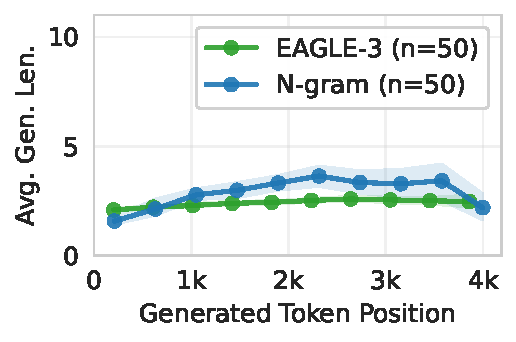
\includegraphics[width=\linewidth]{figures/acc_len/token_level/overlaid_binned_positions_gpqa_main_Qwen3-8B_bin0_range0-4190.pdf}
    \caption{Requests with outputs shorter than 4K tokens}
  \end{subfigure}
    \hspace{1pt}
    \begin{subfigure}{0.45\linewidth}
    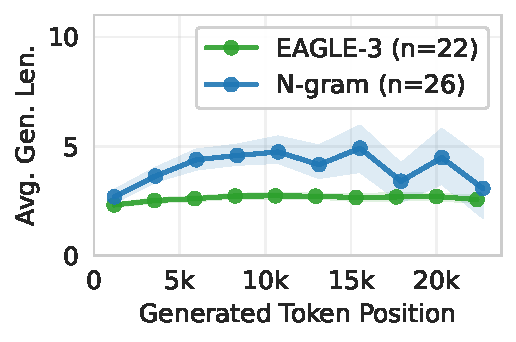
\includegraphics[width=\linewidth]{figures/acc_len/token_level/overlaid_binned_positions_gpqa_main_Qwen3-8B_bin3_range13351-32771.pdf}
    \caption{Requests with outputs longer than 13K tokens}
  \end{subfigure}
  \begin{subfigure}{0.45\linewidth}
    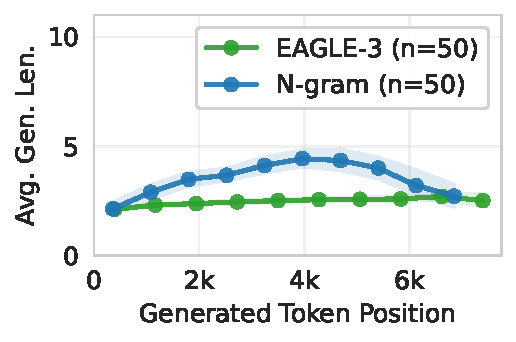
\includegraphics[width=\linewidth]{figures/acc_len/token_level/overlaid_binned_positions_gpqa_main_Qwen3-8B_bin1_range4190-7811.pdf}
    \caption{Requests with outputs of 4K-8K tokens}
  \end{subfigure}
    \hspace{1pt}
    \begin{subfigure}{0.45\linewidth}
    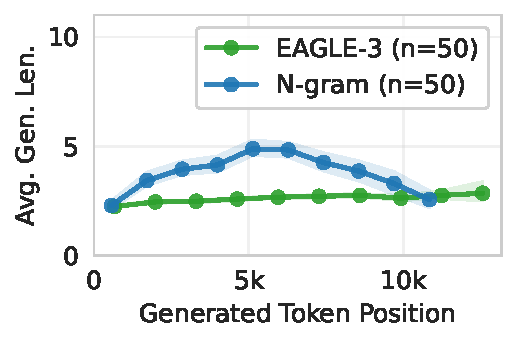
\includegraphics[width=\linewidth]{figures/acc_len/token_level/overlaid_binned_positions_gpqa_main_Qwen3-8B_bin2_range7811-13351.pdf}
    \caption{Requests with outputs of 8K-13K tokens}
  \end{subfigure}
  \vspace{-0.1in}
\caption{Average generation length (tokens) per output token position for Qwen3-8B-Thinking on GPQA-Main. Shaded bands show the 95\% confidence interval.}
  \label{fig:acc-len-token-level}
\end{figure}


\begin{figure} [t!]
  \centering
  
\includegraphics[width=0.8\linewidth]{figures/acc_len/request_level/legend.pdf}

  \begin{subfigure}{0.45\linewidth}
    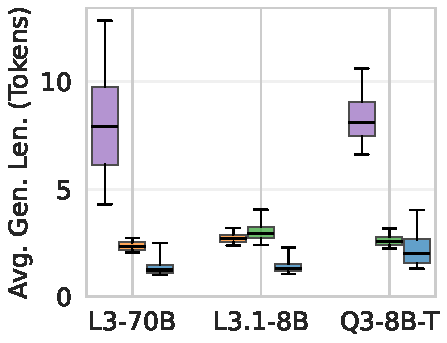
\includegraphics[width=\linewidth]{figures/acc_len/request_level/box_by_model_gsm8k_acc_len.pdf}
    \caption{GSM8K}
  \end{subfigure}
      \hspace{1pt}
    \begin{subfigure}{0.45\linewidth}
    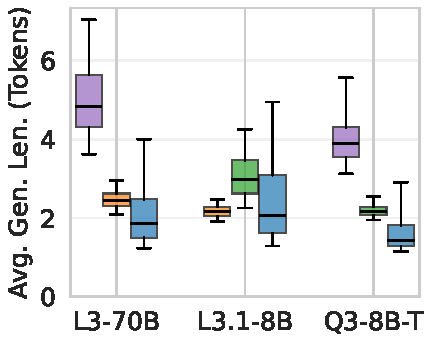
\includegraphics[width=\linewidth]{figures/acc_len/request_level/box_by_model_cnndailymail_acc_len.pdf}
    \caption{CNNDailyMail}
  \end{subfigure}
      \hspace{1pt}
  \begin{subfigure}{0.45\linewidth}
    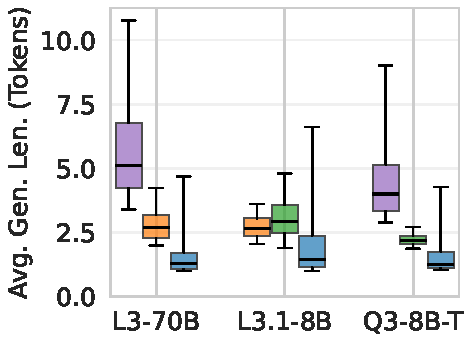
\includegraphics[width=\linewidth]{figures/acc_len/request_level/box_by_model_sharegpt_acc_len.pdf}
    \caption{ShareGPT}
  \end{subfigure}
      \hspace{1pt}
  \begin{subfigure}{0.45\linewidth}
    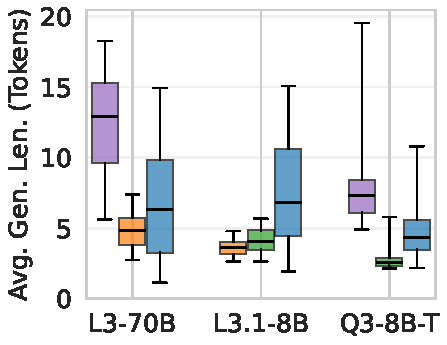
\includegraphics[width=\linewidth]{figures/acc_len/request_level/box_by_model_instructcoder_acc_len.pdf}
    \caption{InstructCoder}
  \end{subfigure}
\caption{Request-level generation length across datasets and models. Each box shows the distribution of per-request mean generation length, with the box spanning the 25th–75th percentiles and whiskers covering the 5th–95th percentiles. Models from left to right are Llama3.1-8B, Llama3-70B and Qwen3-8B-Thinking. Results for reasoning datasets (AIME22–24 and GPQA-Main) are shown in~\autoref{fig:acc-len-request-level-box-plot-reasoning}.}
  \label{fig:acc-len-request-level-box-plot}
\end{figure}



\begin{quoting}[leftmargin=1.5em, rightmargin=1.5em, vskip=0pt]
\textbf{Across Requests and Datasets.}
\emph{Draft-model-based method typically achieves the longest median generation lengths across all workloads, EAGLE attains more stable per-request generation lengths, whereas $n$-gram shows higher variance and a heavy-tailed generation-length distribution.}
\end{quoting}

% \jerry{Updated, please read the entire section again.} 
We observe substantial variance in per-request generation length in \autoref{fig:acc-len-request-level-box-plot}. Even within the same workload, the efficiency of speculative decoding can differ drastically. For example, on InstructCoder with Llama3-70B, EAGLE produces relatively short request-level generation lengths (2.7-7.4 tokens), whereas $n$-gram and draft-model-based SD achieve longer lengths with wider spreads (1.1–15.0 tokens and 5.6-18.3 tokens, respectively). In other workloads (e.g. ShareGPT and CNN/DailyMail) and target models (e.g. Qwen3-8B), draft-model-based methods similarly shows higher generation lengths than $n$-gram and EAGLE.

% Too many data, rewrite this.
% We observe that per-request generation length varies widely in \autoref{fig:acc-len-request-level-box-plot}. 
% Even within the same workload, the efficiency of speculative decoding can differ drastically. On InstructCoder with Llama3-70B, request-level generation lengths span from 1.1–15.0 tokens for $n$-gram (mean 7.0, std 4.3), 2.7-7.4 for EAGLE (mean 4.9, std 1.4) and 5.6-18.3 for Draft-Model-based (mean 12.4, std 3.8). Similar disparities appear in ShareGPT (1.0–4.7 vs.\ 2.0–4.2 vs.\ 3.4-10.8, std 1.6 vs.\ 1.0 vs.\ 2.5), and CNN/DailyMail (1.2–4.0 vs.\ 2.1–3.0 vs.\ 3.6-7.0, std 0.9 vs.\ 0.3 vs.\ 1.0).
% and GSM8K (1.0-2.5 vs.\ 2.0–2.7 vs.\ 4.3-12.9, std  0.5 vs.\ 0.2 vs.\ 2.7), 
% where the average generation length of most requests clusters around 1.5–3 tokens for $n$-gram and eagle. 

These distributions reveal distinct proposal behaviors for each SD variant. Draft-model-based methods often achieve substantially longest generation lengths, but their whiskers (5th-95th percentiles) are also broadly spread. 
% \jerry{@lily, does this explanation sound reasonable to you?} 
The reason behind this may be request-dependent alignment: for some requests, the draft model can track the target model closely so that many proposed tokens are accepted, while for others, it diverges early and only a few draft tokens are accepted after verification.

For $n$-gram, it exhibits heavy tails and large variance across requests, with standard deviations roughly 2x-5x higher than those of EAGLE-based methods. 
While most $n$-gram requests produce short accepted spans, a small subset yield exceptionally long bursts (often exceeding 15 tokens), as seen as long blue strips in \autoref{fig:acceptance-length-heatmap}. 
In code-editing tasks, these typically correspond to locally repetitive content (e.g., reused identifiers, function templates, or class definitions). We select and show an example in \autoref{fig:ngram_prompt_output_full}. Such bursty acceptance behavior reveals that $n$-gram speculation relies on discrete pattern matches that may occur infrequently but can produce large payoffs when present. Consequently, $n$-gram's performance is high when the local contexts are repetitive, but it remains unstable across requests and workloads.


In contrast, EAGLE and EAGLE-3 show compact, symmetric distributions centered near their medians (typically 2–4 tokens), indicating steadier acceptance driven by learned contextual representations rather than surface-level overlap.

These distributional behaviors are consistent with the end-to-end outcomes in \autoref{fig:e2e-speedup}. Draft-model-based methods deliver the largest speedups when the cost of running a separate draft model is relatively low. EAGLE/EAGLE3 follows and provides modest gains on most workloads. $n$-gram achieves its best speedups on highly repetitive code-editing tasks, where rare but very long bursts occur. Outside such settings, its heavy-tailed and unstable acceptance makes performance less predictable.




\begin{figure*}[t]
\centering
\lstset{style=codebox, language=Python}

\begin{minipage}[t]{0.485\textwidth}
\textbf{Prompt}
\begin{lstlisting}
class Car:

    def __init__(self, make, model, year, color):
        self.make = make
        self.model = model
        self.year = year
        self.color = color


car1 = Car('Toyota', 'Camry', 2018, 'Red')
print(car1.color)

# Replace the string data type used for car color with an enum data type. 
# Just output the code, do not include any explanation.
\end{lstlisting}
\end{minipage}\hfill
\begin{minipage}[t]{0.485\textwidth}
\textbf{Output}
\begin{lstlisting}
from enum import Enum


class Color(Enum):
    RED = 1
    BLUE = 2
    GREEN = 3
    YELLOW = 4
    BLACK = 5
    WHITE = 6


class Car:

    def __init__(self, make, model, year, color):
        self.make = make
        self.model = model
        self.year = year
        self.color = color


car1 = Car('Toyota', 'Camry', 2018, Color.RED)
print(car1.color)
\end{lstlisting}
\end{minipage}

\vspace{-0.4em}
\caption{\textbf{Example of prompt-output repetition in code editing from InstructCoder.} The output preserves most of the prompt and applies a localized edit, a structure that $n$-gram can exploit to produce occasional long accepted spans.}
\label{fig:ngram_prompt_output_full}
\vspace{-1.0em}
\end{figure*}
\begin{figure*}[h!]
\begin{center}
\captionsetup{justification=centering}
\begin{subfigure}{0.24\linewidth}
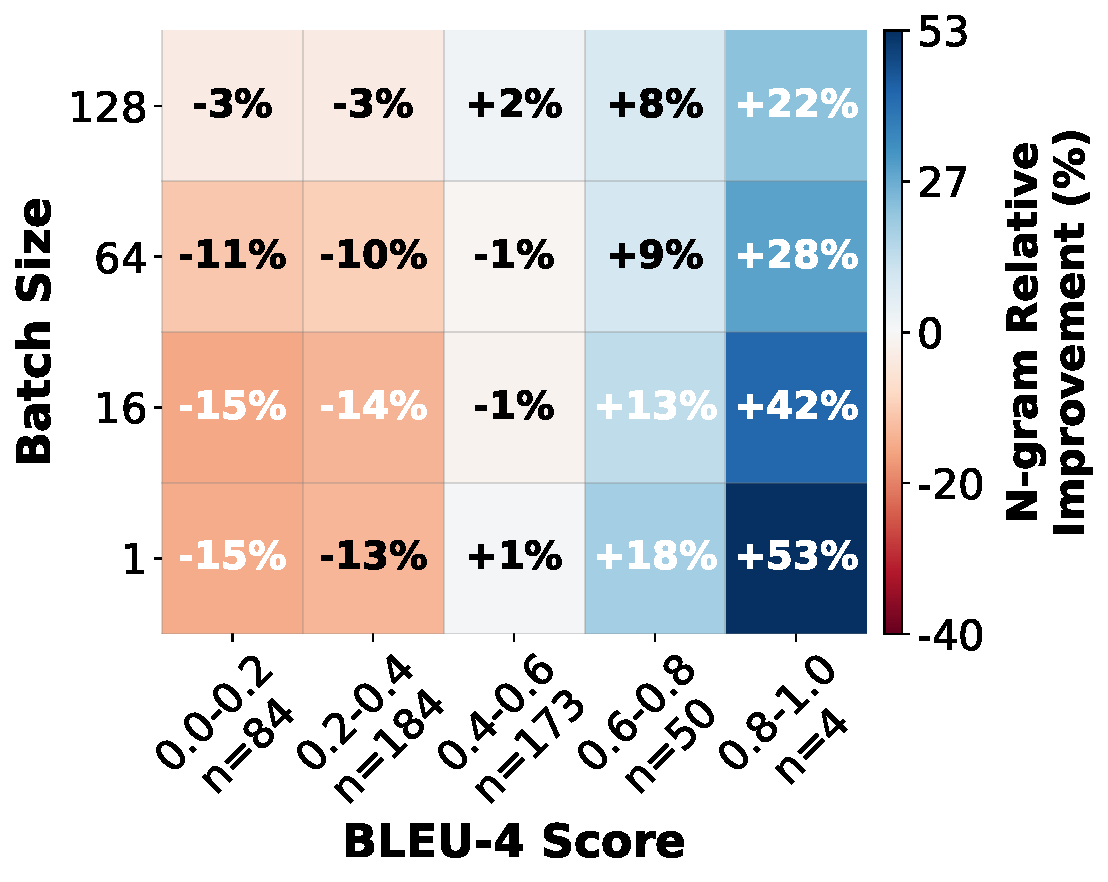
\includegraphics[width=\linewidth]{figures/BLEU_Score/instructcoder_meta-llama_Llama-3.1-8B-Instruct_ngram_vs_eagle_relative_heatmap.pdf}
\caption{Llama3.1-8B, $n$-gram-fixed-3 vs EAGLE}
\end{subfigure}
\begin{subfigure}{0.24\linewidth}
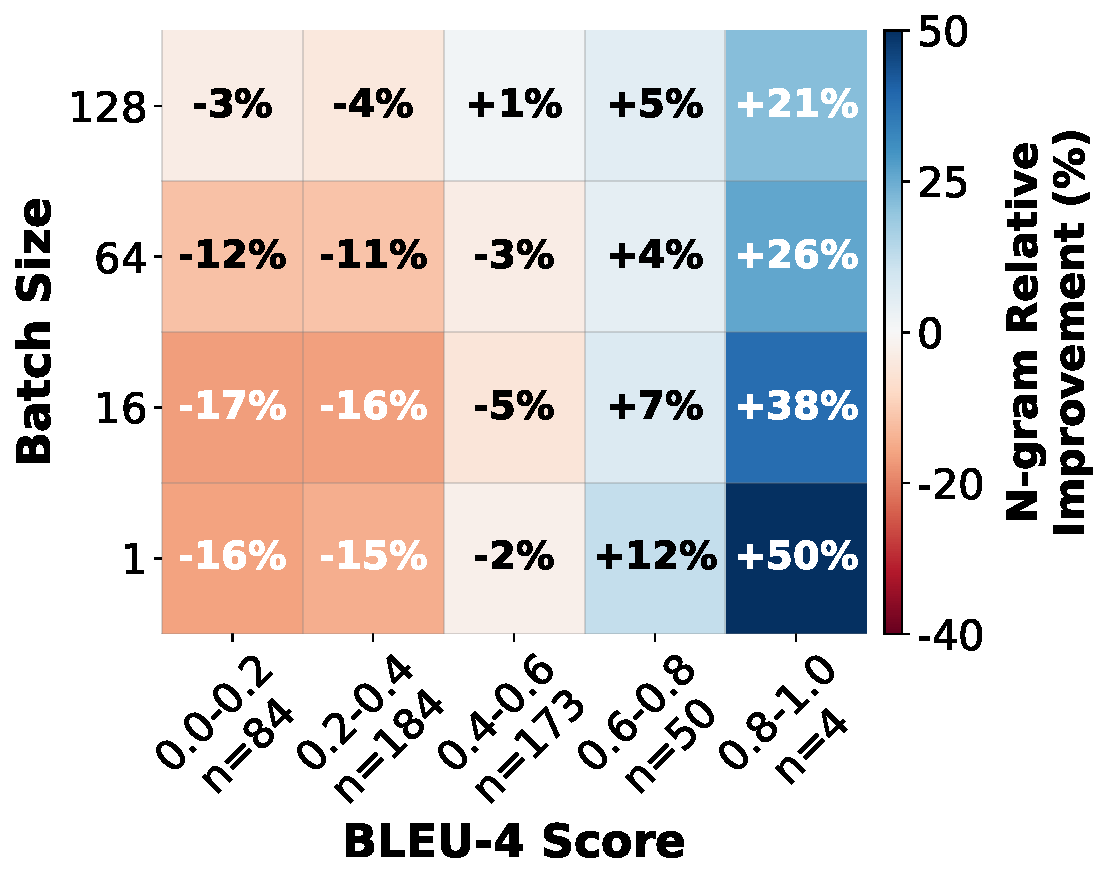
\includegraphics[width=\linewidth]{figures/BLEU_Score/instructcoder_meta-llama_Llama-3.1-8B-Instruct_ngram_vs_eagle3_relative_heatmap.pdf}
\caption{Llama3.1-8B, $n$-gram-fixed-3 vs EAGLE-3}
\end{subfigure}
\begin{subfigure}{0.24\linewidth}
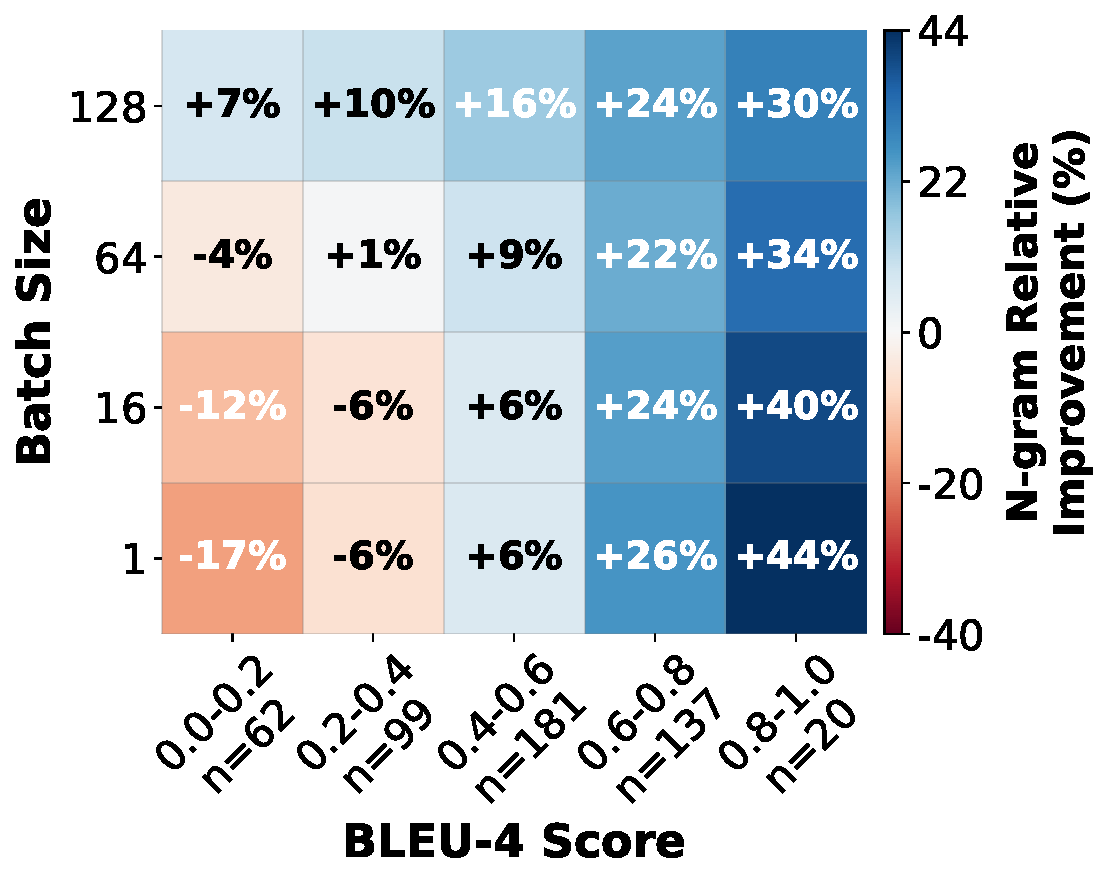
\includegraphics[width=\linewidth]{figures/BLEU_Score/instructcoder_Qwen_Qwen3-8B_ngram_vs_eagle3_relative_heatmap.pdf}
\caption{Qwen3-8B, $n$-gram-fixed-3 vs EAGLE-3}
\end{subfigure}
\begin{subfigure}{0.24\linewidth}
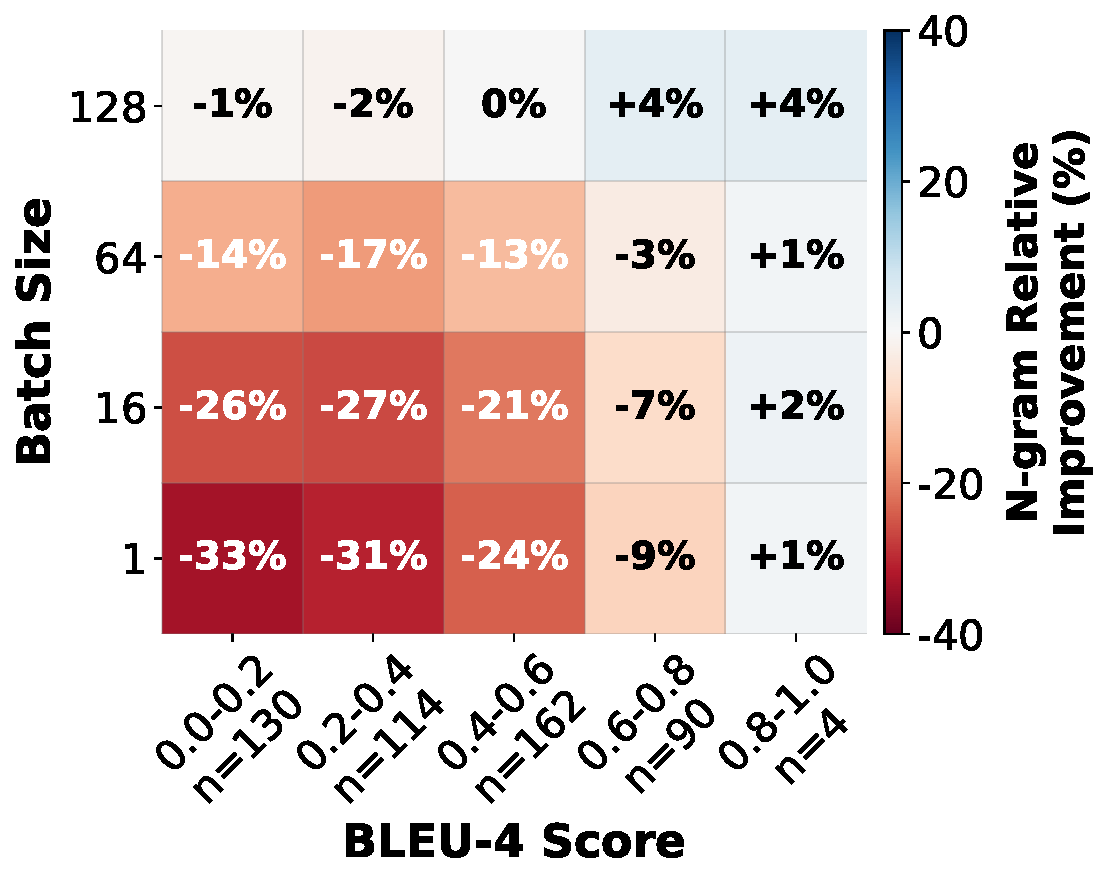
\includegraphics[width=\linewidth]{figures/BLEU_Score/instructcoder_meta-llama_Meta-Llama-3-70B-Instruct_ngram_vs_eagle_relative_heatmap.pdf}
\caption{Llama3-70B, $n$-gram-fixed-3 vs EAGLE}
\end{subfigure}

% NRGAM-FIXED-5 Below
\begin{subfigure}{0.24\linewidth}
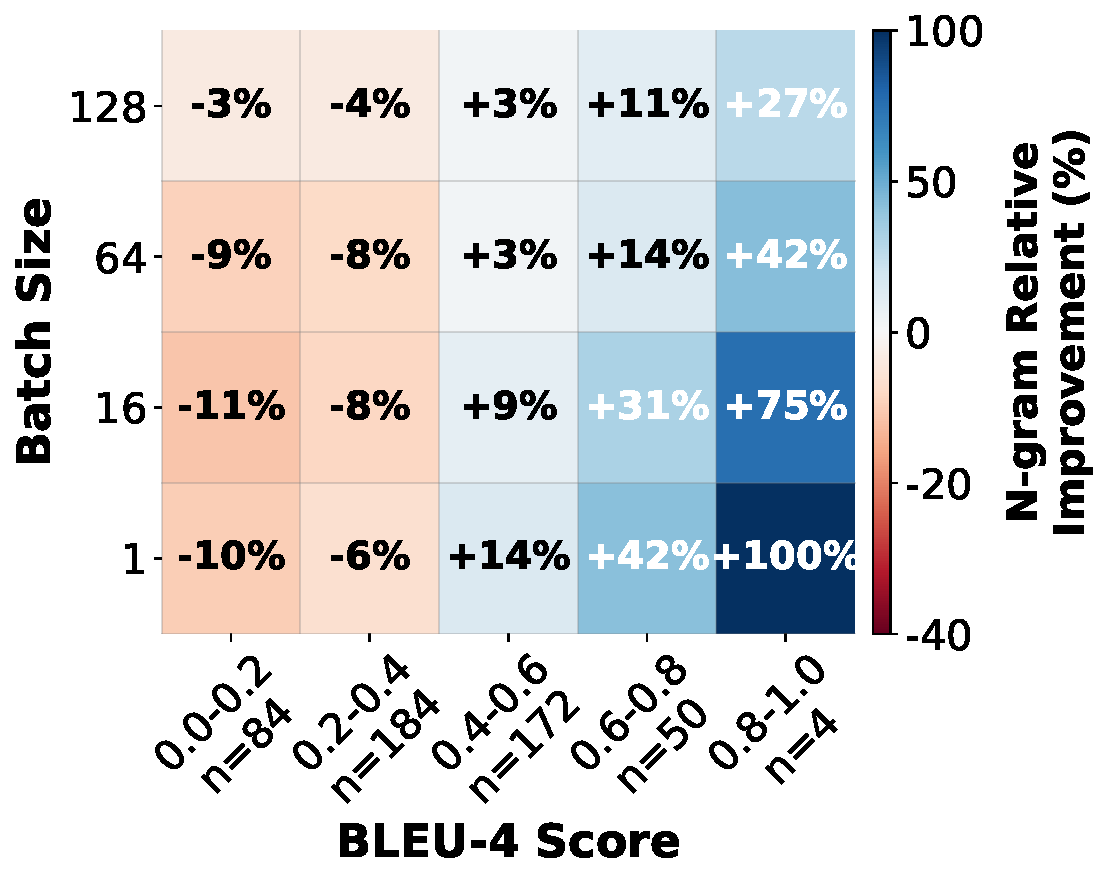
\includegraphics[width=\linewidth]{figures/BLEU_Score/ngram5-reduced-batchsize/instructcoder_meta-llama_Llama-3.1-8B-Instruct_ngram_vs_eagle_relative_heatmap.pdf}
\caption{Llama3.1-8B, $n$-gram-fixed-5 vs EAGLE}
\end{subfigure}
\begin{subfigure}{0.24\linewidth}
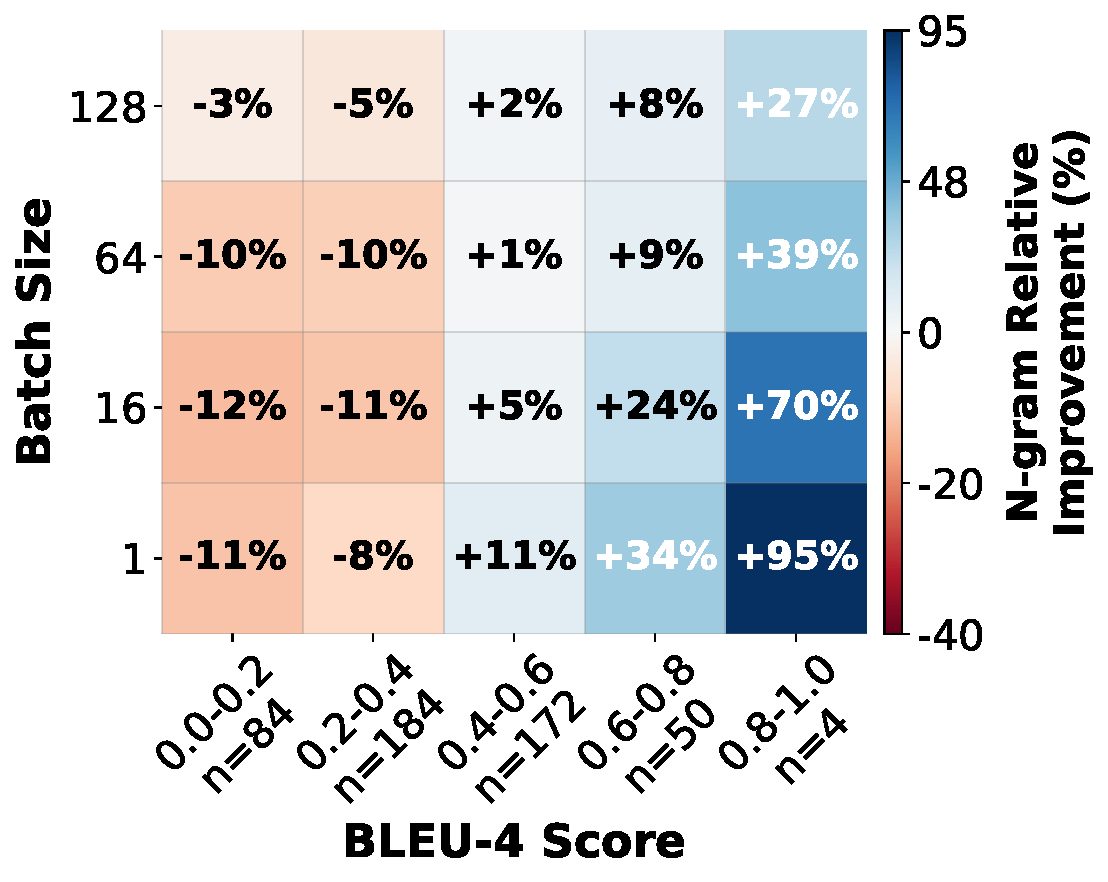
\includegraphics[width=\linewidth]{figures/BLEU_Score/ngram5-reduced-batchsize/instructcoder_meta-llama_Llama-3.1-8B-Instruct_ngram_vs_eagle3_relative_heatmap.pdf}
\caption{Llama3.1-8B, $n$-gram-fixed-5 vs EAGLE-3}
\end{subfigure}
\begin{subfigure}{0.24\linewidth}
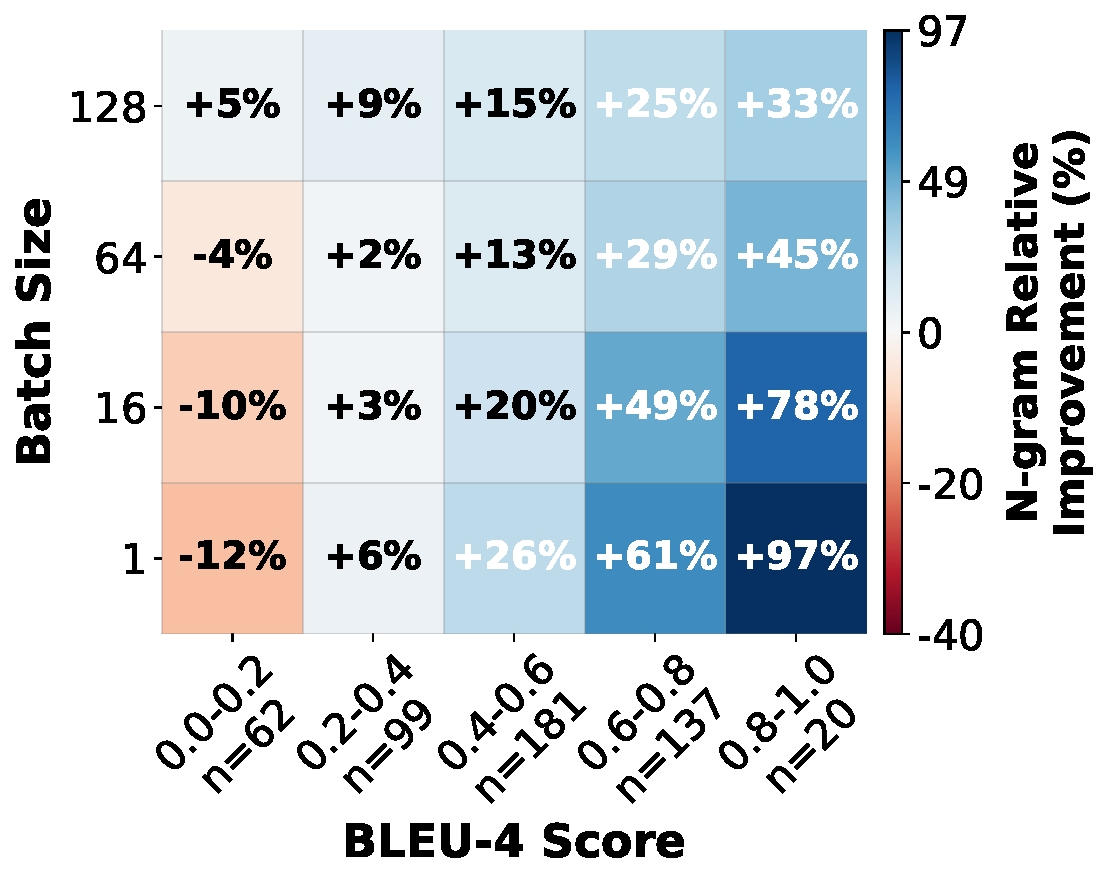
\includegraphics[width=\linewidth]{figures/BLEU_Score/ngram5-reduced-batchsize/instructcoder_Qwen_Qwen3-8B_ngram_vs_eagle3_relative_heatmap.pdf}
\caption{Qwen3-8B, $n$-gram-fixed-5 vs EAGLE-3}
\end{subfigure}
\begin{subfigure}{0.24\linewidth}
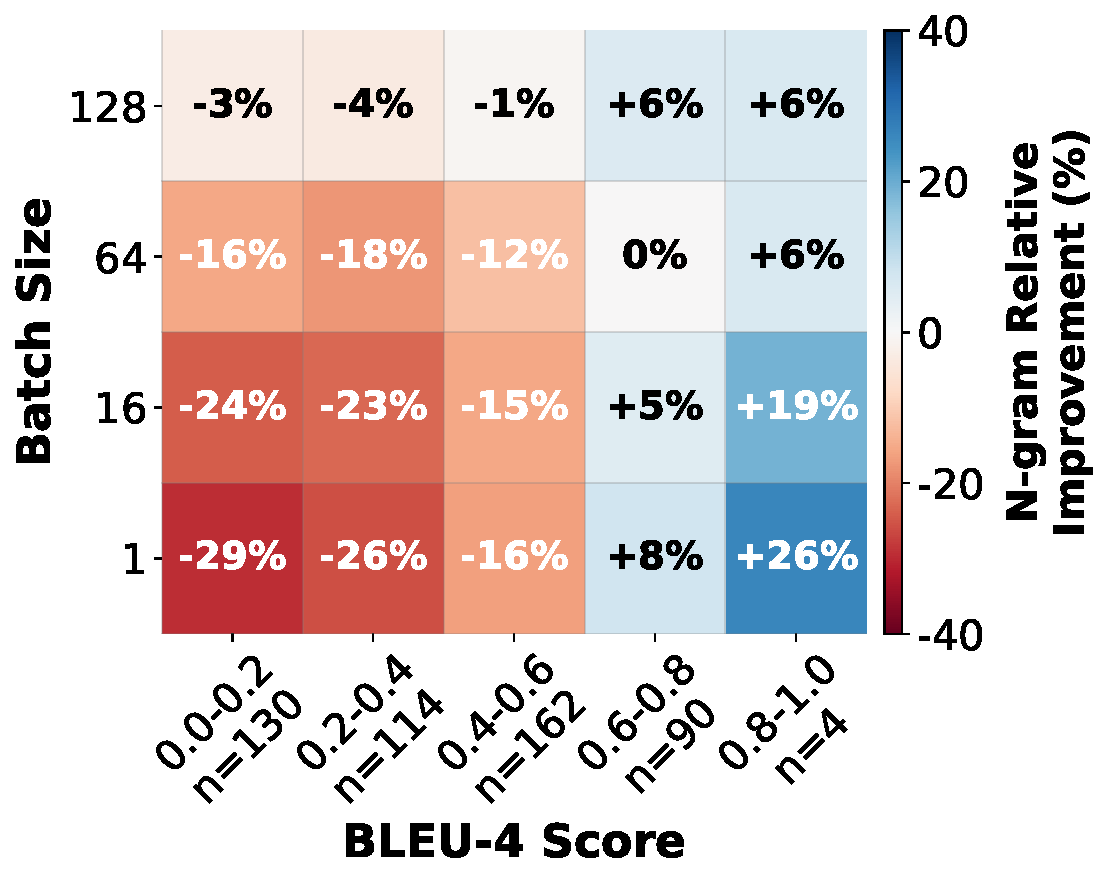
\includegraphics[width=\linewidth]{figures/BLEU_Score/ngram5-reduced-batchsize/instructcoder_meta-llama_Meta-Llama-3-70B-Instruct_ngram_vs_eagle_relative_heatmap.pdf}
\caption{Llama3-70B, $n$-gram-fixed-5 vs EAGLE}
\end{subfigure}

\caption{Correlation between BLEU-4 and $n$-gram speedup on InstructCoder. Each heatmap shows $n$-gram’s relative speedup (\%) over EAGLE or EAGLE-3, grouped by BLEU-4 scores (x-axis) and batch sizes (y-axis). Blue means that $n$-gram outperforms the draft-model method, while red means the opposite. $n{=}$XYZ in the x-axis labels denotes the number of requests in each BLEU bucket. Figures (a) to (d) show the results when $n$-gram proposes 3 tokens per step and Figures (e) to (h) show the results when that is set to 5.}
\label{fig:ngram_bleu_heatmap}
\vspace{-0.2in}
\end{center}
\end{figure*}

